\chapter{State of the Art}\label{StateOfTheArt}
In this chapter we will go over the latest improvements for CNNs. 
They range from the activation function used within each neuron to major architecture changes to combat problems that arise from training deeper and deeper networks.


\section{Activation Functions}
The current trend has been using activation functions that are non-saturated, meaning they do not have very small derivatives at large input values. 
Also, these new functions are chosen to help combat the `vanishing gradient problem' \cite{hochreiter2001gradient}.
This problem was due to many of the originally used activation functions (e.g sigmoid or tanh) 'squash' their input into a very small output range in a very non-linear fashion. 
For example, sigmoid maps the real number line onto a `small' range of $[0, 1]$. 
As a result, there are large regions of the input space which are mapped to an extremely small range. 
In these regions of the input space, even a large change in the input will produce a small change in the output - hence the gradient is small.
This becomes much worse when we stack multiple layers of such non-linearities on top of each other, leading to difficulty in training deeper networks.
We will go through a few new activation functions, whose plots are shown in Fig.~\ref{f:activations}.

\paragraph{ReLU:}
The most notable non-saturated activation function is the rectified linear unit (ReLU) \cite{nair2010rectified}. 
This is defined as:
\begin{equation}
f(x) = \mbox{max}(0,x).
\label{e:relu}
\end{equation}
The benefits of this unit include: faster calculation since the max($\cdot$) operation is faster than sigmoid or tanh, it creates sparsity in the hidden units by giving true zero values often to help sparse representations form, and does not suffer from vanishing gradients in deep models. 
The vanishing gradient problem



ReLU has been shown to work better than sigmoid or tanh in several tasks and shows fast convergence even without pretraining \cite{glorot2011deep,krizhevsky2012imagenet,zeiler2013rectified,maas2013rectifier}.

\paragraph{LReLU:}
The ReLU has zero gradient whenever its inputs add to a negative value or when a large gradient changes the weights to large negatives value making future input into the unit always have a negative value. 
These units will never be updated and learning will not occur, which can be a problem. 
Mass \textit{et al}. 
\cite{maas2013rectifier} found a solution to this by introducing a non zero component to the ReLU when the input is negative. 
They called this unit the Leaky ReLU as it 'leaks' a positive gradient on the negative side of its graph by having a very small slope. 
This leaky ReLU or LReLU is defined as:
\begin{equation}
f(x) = \mbox{max}(0,x) + \lambda ~\mbox{min}(0,x)
\label{e:lrelu}
\end{equation}
where $\lambda \in (0,1)$ and is predefined per model. 
This unit allows for small gradients when the unit is not active, which helps the problems of the ReLU unit.

\paragraph{PReLU:}
Rather than trying to find an optimal value for $\lambda$ in the LReLU, He et al. \cite{he2015delving} introduced the Parametric ReLU which adapts the $\lambda$ during training. 
It is defined as:
\begin{equation}
f(x) = \mbox{max}(0,x) + \lambda_k ~\mbox{min}(0,x)
\label{e:prelu}
\end{equation}
where $\lambda_k$ is the $k$-th channel. 
Since the number of parameters in networks is often very large compared to the number of total channels, the extra computational cost to learn the values of $\lambda_k$'s is not much.

\paragraph{ELU:}
Next is the Exponential Linear Unit (ELU) \cite{clevert2015fast}. 
ELUs are similar to the above mentioned units, but they have a saturating function on their negative side. 
The saturation function decreases the variation of the units if they are not activated, which gives those units a chance to update while making them more robust to noise. 
The ELU function is defined as:
\begin{equation}
f(x) = \mbox{max}(0,x) + \mbox{min}(0,\lambda(e^{x}-1))
\label{e:elu}
\end{equation}
where $\lambda$ is predefined as in the LReLU.

\paragraph{PELU:}
A natural extension of the ELU is the Parametric ELU \cite{trottier2016parametric}. 
Unlike the PReLU which learns one parameter to modify the LReLU, the PELU learns two parameters during training to modify the ELU. 
This gives the network more control over the vanishing gradients. 
The PELU is defined as:
\begin{equation}
f(x) = \mbox{max}(0,\frac{a}{b}x) + \mbox{min}(0,a(e^{x/b}-1))
\label{e:pelu}
\end{equation}
where $a,b > 0$. 
Both $a$ and $b$ change the slope of the linear function together, $b$ effects the scale of the exponential decay, and $a$ is the saturation point in the negative side of the function. 
In \cite{trottier2016parametric} it is shown that PELU does a better job than all the above functions in several different models and data sets.

\begin{figure}[h!]
	\centering
		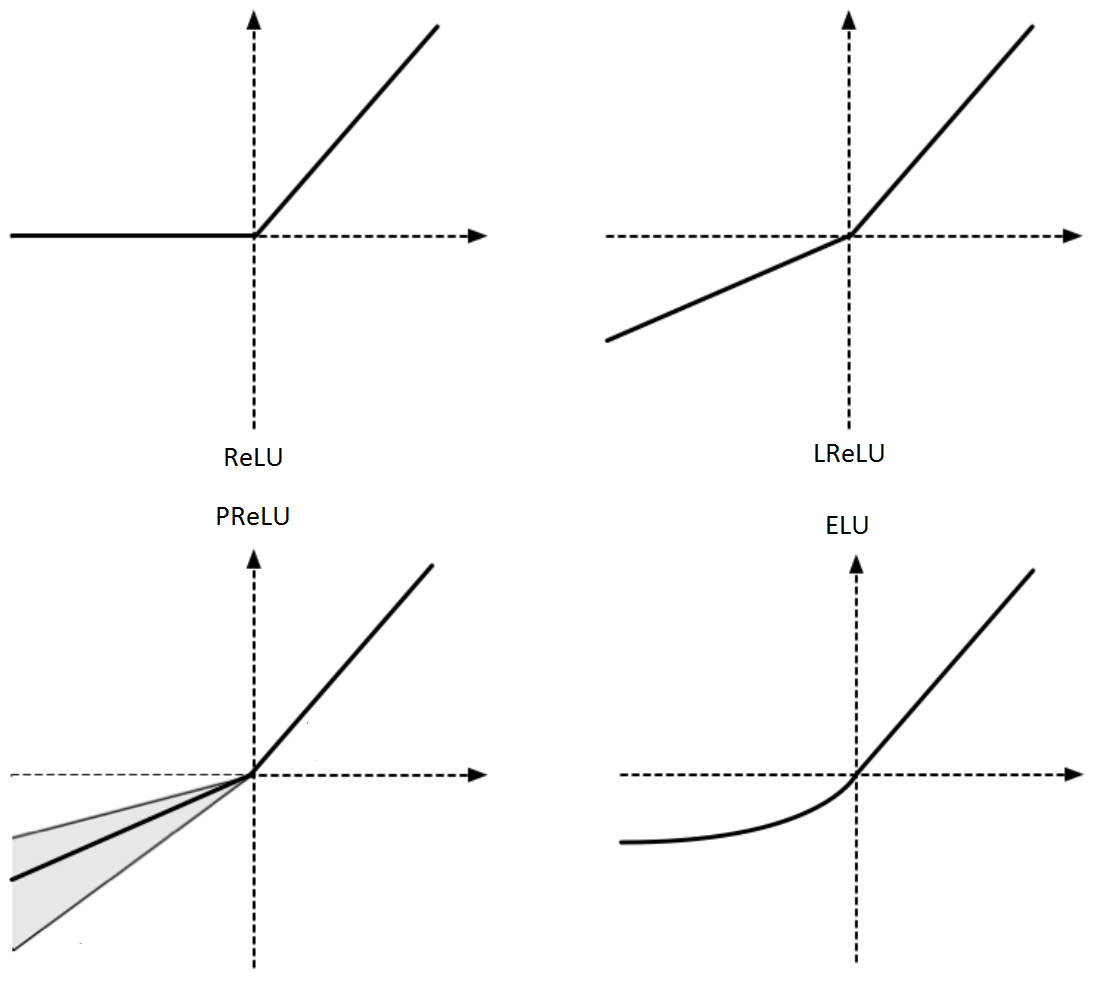
\includegraphics[width=0.85\textwidth]{figures/activations.png}
	\caption{Examples of some of the discussed activation functions. From top to bottom and left to right: ReLU, LReLU, PReLU, and ELU. \cite{}}
	\label{f:activations}
\end{figure}


\section{Regularization}
Some of the biggest improvements to NNs have been through regularizing the network in different ways to prevent overfitting.
Overfitting means that the network learns the training set well, but performs poorly on any new or unseen data.

\paragraph{Dropout:}
Introduced by Hinton \textit{et al.} \cite{hinton2012improving}, Dropout has shown to be very effective at improving network results and reducing overfitting. 
In their paper Dropout is applied to fully-connected layers where the output of the Dropout layer is 
\begin{equation}
\textbf{y} = \textbf{r} \ast a(\textbf{W}^T\textbf{x}), 
\label{eq:dropout}
\end{equation}
where $\textbf{x} = [x_1,x_2,...,x_n]^T$ is the input to the fully-connected layer, $a(\cdot)$ is an activation function, $\textbf{W}$ is the weight matrix, $\ast$ is an element-wise multiplication, and $\textbf{r}$ is a binary vector whose elements are independently drawn from a Bernoulli distribution with parameter $p$. 
This means that at every update to the network, each neuron has a $p$ chance of getting multiplied by zero. 
Dropout usually prevents the network from becoming too reliant on a few neurons and helps the network generalize by spreading feature information. 
Some extensions to Dropout have been proposed like in \cite{wang2013fast} where a method to improve the speed of training while using Dropout are introduced. 
Similar to the learned parameters of the activation functions, \cite{ba2013adaptive} learn the $p$ in the Dropout distribution adaptively. 
Finally, in \cite{tompson2015efficient} they modify Dropout with CNNs specifically in mind by extending the Dropout value across the entire feature map, meaning that during training each feature map has a $p$ chance of being completely ignored for each update step. 
They call this method Spatial Dropout and it seems to help the network learn more general features, which improves results on limited size data sets.

\paragraph{Batch Normalization:}
It is standard practice to normalize data to have zero-mean and unit variance before feeding it into a NN, but as the data goes through the network, especially deep networks, the data will lose this property. 
This change to the input distribution is known as internal covariance shift. 
To keep data normed through the network \cite{ioffe2015batch} introduced an efficient method called Batch Normalization (BN). 
BN works by normalizing the mean and variance of each layers input using each batch rather than the entire training set. 
To demonstrate BN, let $\textbf{x} = [x_1,x_2,...,x_n]^T$ be a $n$ dimensional input to a layer. 
The $k$-th dimensions is normalized by:
\begin{equation}
\hat{x}_k = (x_k - \mu_{B})/\sqrt{\sigma^2_B + \epsilon}
\label{eq:BN1}
\end{equation}
where $\mu_{B}$ and $\sigma^2_B$ are the mean and variance of the batch respectively and $\epsilon$ is some small constant value that will guarantee the root term is always defined. 
Finally the input $\hat{x}_k$ is further transformed:
\begin{equation}
y_k = \mbox{BN}_{\alpha,\beta}(x_k) = \alpha \hat{x}_k + \beta
\label{eq:BN2}
\end{equation}
where $\alpha$ and $\beta$ are parameters learned during training. 
There are many benefits to using BN. 
By reducing internal covariance shift the network will converge faster. 
By making sure no inputs get too large or small BN makes it possible to use saturating activation functions without fear of getting stuck in a saturating section and having vanishing gradients.

\section{Architecture Improvements}
There are a couple of recent architecture improvements to NNs that both help with speed (by lowering computational cost for similar results) and immensely with vanishing gradients.

\paragraph{Network-In-Network} 
The first was introduced in \cite{lin2013network} where they use fully connected layers on the outputs of each convolution operation called Network-in-network. 
The idea was an alternative to stacking multiple convolutional layers (each with a number of their own filters) to get deepness in a neural network model, by replacing each filter with a multi-layer perceptron, which is essentially a small neural network that slides across the image like a convolutional filter. 
The math works out so that a $1\times 1\times U$ convolution filter convolved across a $V$-channel image emulates a $U\times V$ matrix multiplied by each $V$-channel pixel, which is the same as running a single-layer neural network across every pixel of your input as if each pixel were an example vector in a training set. 
Chaining together such $1\times 1\times U$ convolutions, you get the same result as if running a many-layered neural network at each input pixel of $V$ channels. 
The idea from the paper was to turn a convolution filter which is a generalized linear model, into a non-linear model. 
It allows the network to combine channels from previous layer in a non-linear fashion, which can lead to more advanced features.

\paragraph{Inception Blocks}
Google's team was inspired by the Network-in-network paper and saw the power of using the 1x1 convolutions not only for non-linearaity, but to reduce computational burden of deep models by using the cross-channel pooling aspect to reduce their feature maps before convolution layers. 
In \cite{szegedy2015going} Christian Szegedy and his team introduced the Inception module as seen in Fig.\ref{f:inceptionblock}. 
\begin{figure}[h!]
	\centering
		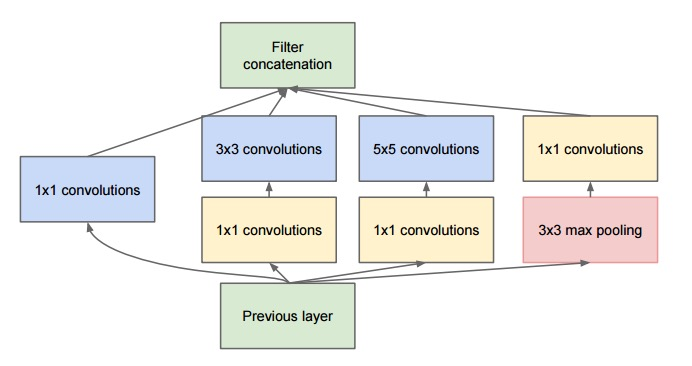
\includegraphics[width=1.0\textwidth]{figures/inceptionblock.png}
	\caption{An inception block from \cite{szegedy2015going}. Notice the 1x1 convolutions before the 3x3 and 5x5 convolutions are reducing the number of feature channels. This reduces the number of multiplications that must be performed.}
	\label{f:inceptionblock}
\end{figure}

\paragraph{Residual Connections}
Another work that focused on fixing the vanishing gradient problem of deep networks was Residual Nets (ResNets) \cite{he2015deep} where they used what is now called shortcut connections. 
These connections were inspired by Long Short Term Memory (LSTM) units, a type of recurrent neural network unit that feeds information back into itself with weighted gates. 
Instead of using weighted gates shortcut connections pass information with the identify function so it is untransformed. 
This means that the activation of deep units can be written as the sum of the activation of some shallower unit and a residual function, which is a series of network layers. 
Or to put simply, the input to a layer group is added to the output of that layer group. 
This is called a Residual Block and can be seen in Fig.\ref{f:resblock}. 
By stacking these residual blocks together one gets a fully residual model. 
This design allows the gradients to be directly propagated to shallower units allowing for networks of 100s of layers to be trained. 
\begin{figure}[h!]
	\centering
		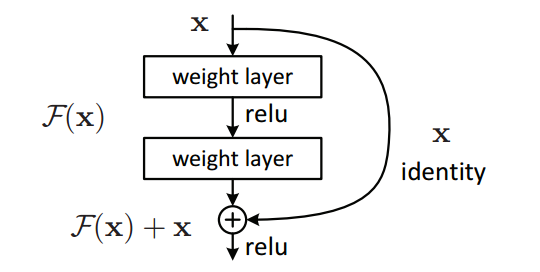
\includegraphics[width=0.80\textwidth]{figures/resblock.png}
	\caption{A residual block from \cite{he2015deep}.}
	\label{f:resblock}
\end{figure}


\section{Open Questions}
At present, the vast majority of all work done in neural networks is based on real-valued operations and representations.
There have been some recent work exploring the use of complex numbers and very few the use of hyper-complex number (quaternions) showing promising results due to these numbers having greater representational power to the reals.
In \cite{trabelsi2017deep} they present the first complex forms of complex batch-normalization and complex weight initialization strategies to use along with complex convolution to create a fully complex deep convolutional network.
They achieve some state-of-the-art results over the real-valued counter part models, which leads to the question of creating forms for quaternion batch-normalzation and weight initialization for potentially better results.
